\documentclass[10pt,a4paper]{article}

\usepackage{fontspec}
\setmainfont{Liberation Sans}
\setsansfont{Liberation Sans}
\setmonofont{DejaVu Sans Mono}[Scale=0.86]
\renewcommand{\familydefault}{\sfdefault}
\usepackage{microtype}
\usepackage[a4paper,top=1.5cm,bottom=1.6cm,left=1.9cm,right=1.9cm]{geometry}
\usepackage{graphicx}
\usepackage{xcolor}
\usepackage{booktabs}
\usepackage{enumitem}
\usepackage{parskip}
\usepackage[hidelinks]{hyperref}

\definecolor{ink}{HTML}{10151B}
\definecolor{accent}{HTML}{1F6FEB}
\definecolor{soft}{HTML}{5A6673}
\definecolor{rule}{HTML}{D6DCE3}
\definecolor{panel}{HTML}{F3F6FA}

\pagestyle{empty}
\setlength{\parindent}{0pt}
\setlist[itemize]{leftmargin=1.1em,itemsep=1pt,topsep=2pt,parsep=0pt}

\newcommand{\sectionhead}[1]{%
  \vspace{7pt}%
  {\color{accent}\bfseries\large #1}\\[-6pt]
  {\color{accent}\rule{\linewidth}{0.7pt}}\vspace{3pt}%
}

\begin{document}

% ---------------------------------------------------------------- header
{\color{ink}\bfseries\fontsize{24}{27}\selectfont Newton}\hfill
{\color{soft}\small High-Up! Hackathon \textbullet{} 19--20 November}\\[1pt]
{\color{accent}\bfseries\large A physics visualizer for the classroom}\\[-2pt]
{\color{rule}\rule{\linewidth}{1.1pt}}

\vspace{4pt}
{\small\color{ink}
Physics teachers spend hours drawing the same free-body diagrams, and students still
cannot see the forces changing while the system moves. Newton turns a plain-language
description of a physical system into a live, time-evolving visualization: bodies,
joints, the forces acting on each body, and the energy budget as it unfolds.}

% ---------------------------------------------------------------- problem
\sectionhead{The problem}

\begin{itemize}
  \item \textbf{Diagrams freeze time.} A static free-body diagram shows one instant.
  Students memorize arrows instead of seeing \emph{when} and \emph{why} they change.
  \item \textbf{Simulation tools are expert tools.} Existing physics engines want code,
  scene files and a build step; PhET-style applets are polished but closed --- you cannot
  ask for \emph{your} problem, the exact ramp angle from chapter 7.
  \item \textbf{Teachers have no fast path from a problem statement to a visual.}
  Preparing a demo is a separate project from preparing the lesson.
\end{itemize}

{\color{soft}Newton targets the gap: \textbf{expressive} enough for a specific textbook
exercise, \textbf{fast} enough to use live in class, and \textbf{reliable} enough that a
wrong answer is never silently displayed.}

% ---------------------------------------------------------------- how it works
\sectionhead{How it works}

\begin{center}
  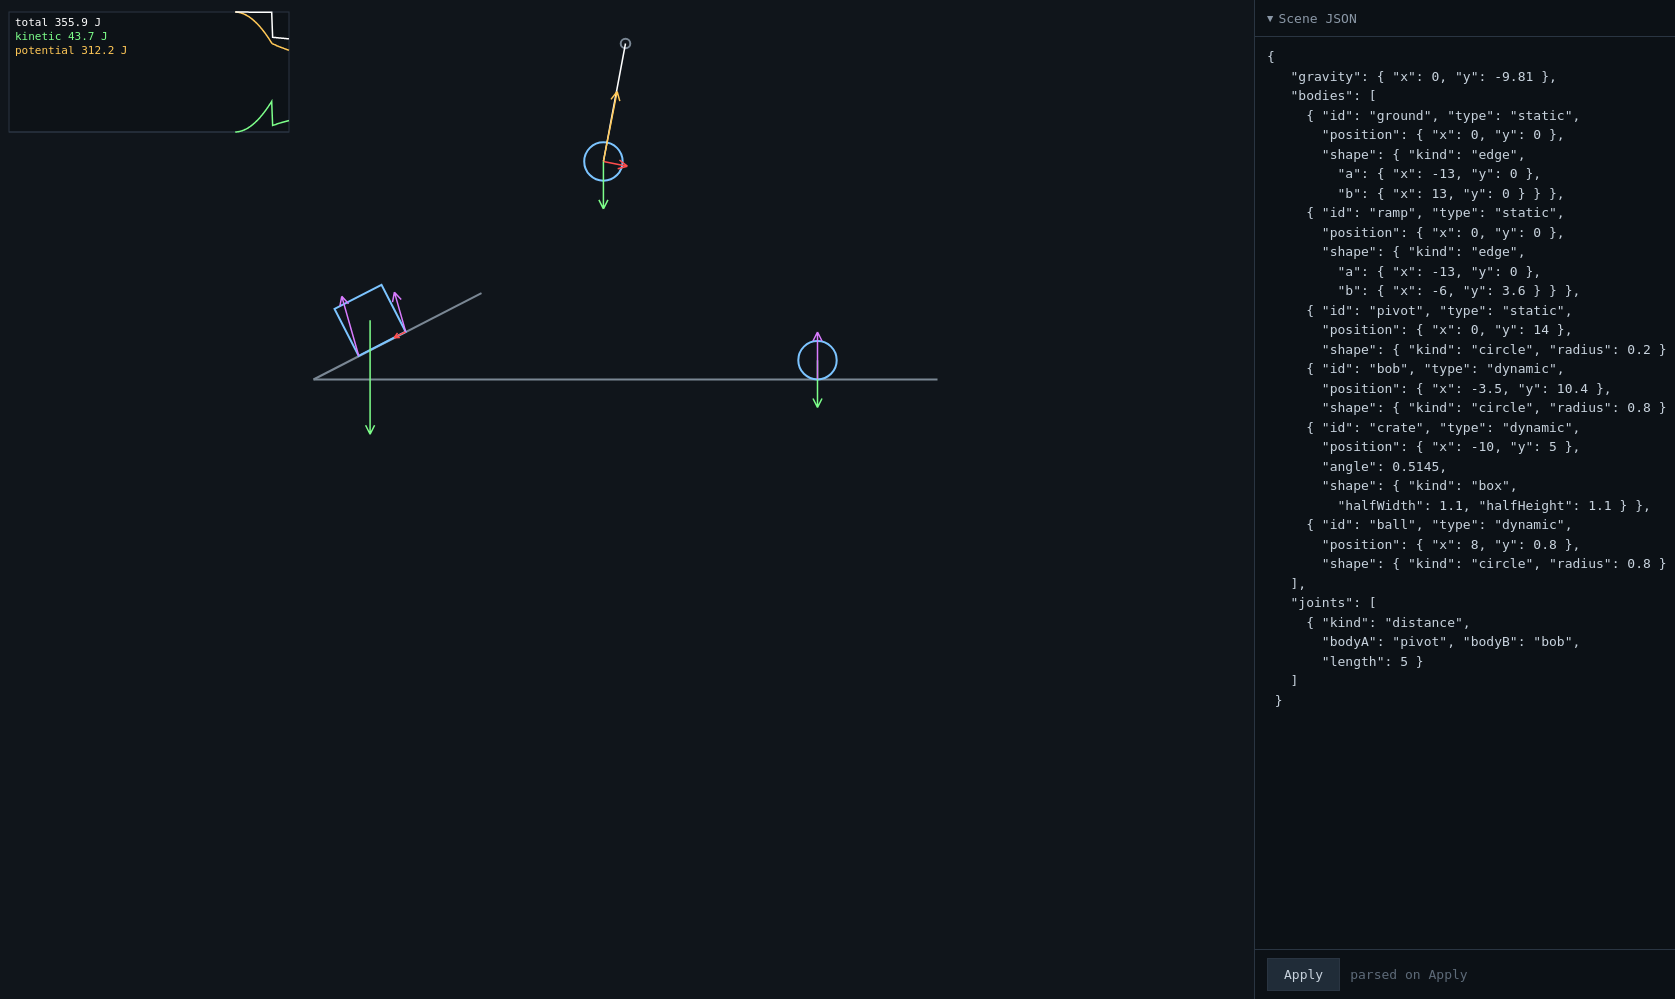
\includegraphics[width=\linewidth]{newshot.png}
\end{center}
{\small\color{soft}\textbf{Current build, running.} A pendulum released at an angle, a crate
resting on a ramp, and a ball on the ground. Green arrows are gravity, ochre the joint
reaction, magenta the normal force from the ramp and ground, red the velocity; the panel
top-left plots kinetic, potential and total energy over the last 5 seconds. The right-hand
pane is the scene document being edited.

\vspace{3pt}
A scene is JSON describing bodies (\texttt{circle}, \texttt{box}, \texttt{edge}), their
mass, shape and pose, and joints between them --- all SI units, $+y$ up, anchors local to
their body so a joint stays attached when the body moves. The document travels through three
gates, and any failure names \emph{every} problem with its path
(\texttt{bodies[1].shape.radius}) so it can be fixed in one pass:}

\begin{enumerate}[leftmargin=1.4em,itemsep=1pt,topsep=2pt,parsep=0pt]
  \item \textbf{Syntax} --- a schema rejects unknown keys, missing positions, malformed shapes.
  \item \textbf{Semantics} --- unique ids, joints that reference real bodies, no zero-area
  dynamic bodies that the engine would silently give a default mass.
  \item \textbf{World} --- the validated document becomes a running simulation at a fixed
  1/120\,s step, decoupled from the frame rate so the physics is the same on a laptop and a
  projector.
\end{enumerate}

\newpage

% ---------------------------------------------------------------- progress
\sectionhead{Current progress}

\begin{center}
\small
\begin{tabular}{@{}p{0.46\linewidth}p{0.46\linewidth}@{}}
\toprule
\textbf{Working today} & \textbf{Deliberately deferred}\\
\midrule
Rigid-body simulation (planck.js) at a fixed 1/120\,s step &
Forces beyond joints, gravity and contacts\\
Scene document with schema + semantic validation &
Compound bodies, springs, friction models\\
Circles, boxes, edges; static and dynamic bodies &
More joint kinds (revolute, prismatic, weld)\\
Distance joints with local anchors &
Saving and sharing scenes (persistence)\\
Live force vectors: gravity, joint reaction, normal &
Natural-language (\emph{``a 2\,kg block on a 30\textdegree{} ramp''}) input\\
Kinetic + potential energy, plotted over time &
Multi-user gallery of published visualizations\\
Pluggable renderer contract (frame $\to$ backend) &
Audio, 3D, mobile layouts\\
JSON editor with hot-reload; errors listed, never swallowed &
\\
\bottomrule
\end{tabular}
\end{center}

\vspace{2pt}
{\small\color{soft}The sim and the renderer are already separate: a frame is a fresh plain
value, so a second backend (WebGL, SVG, export) is one new file and no changes to the physics.
The whole test suite runs headless --- 57 checks covering parsing, validation, joint
behaviour and the frame contract.}

% ---------------------------------------------------------------- roadmap
\sectionhead{Roadmap}

\begin{center}
\small
\begin{tabular}{@{}p{0.13\linewidth}p{0.53\linewidth}p{0.26\linewidth}@{}}
\toprule
\textbf{Phase} & \textbf{Goal} & \textbf{Done when}\\
\midrule
\textbf{Now} & Simulation, validation, force and energy display, JSON editing &
Hackathon demo\\
\textbf{1 --- Express} & More primitives: springs (Hooke's law integrated by hand),
friction forces, applied forces, revolute/prismatic joints, compound shapes &
A pendulum with a spring and a friction ramp is one short document\\
\textbf{2 --- Natural language} & A prompt becomes a scene document. The model writes JSON
only; the validator is the safety net, so an incoherent description is rejected with paths
instead of rendered as nonsense &
``A 2\,kg block slides down a 30\textdegree{} ramp'' plays, with no code\\
\textbf{3 --- Share} & Named scenes, a URL per visualization, a gallery to browse and fork
someone else's system &
A teacher sends a link, a student opens it\\
\textbf{4 --- Classroom} & Guided lesson mode: checkpoints, questions pinned to a moment in
time, and a view students can drive themselves &
A full lesson runs from one link\\
\bottomrule
\end{tabular}
\end{center}

% ---------------------------------------------------------------- objectives
\sectionhead{Objectives and why it matters}

\vspace{-2pt}
{\small
\begin{itemize}
  \item \textbf{Minutes, not hours.} From a textbook sentence to a moving picture in under a
  minute --- short enough to do it live, in front of a class.
  \item \textbf{Robust on stage.} A demo that says \emph{why} it cannot run is worth more in a
  classroom than one that shows a plausible lie. Every invalid input is rejected with a
  readable path; the previous scene keeps playing.
  \item \textbf{Open and inspectable.} The scene is data, the physics is a documented engine,
  the source is GPL-3.0. A teacher can hand the document to a colleague, and a student can see
  there is no magic.
  \item \textbf{A foundation, not a toy.} Forces and energy are exposed through one
  renderer-agnostic contract, so sharing, AI authoring and new backends are additive work
  rather than rewrites.
\end{itemize}}

\vspace{6pt}
{\color{rule}\rule{\linewidth}{0.7pt}}\\[2pt]
{\small\color{soft}
\textbf{Technical status at time of writing} --- 57 passing tests, headless, no network
calls; TypeScript strict; scene schema and validation complete for the current primitives;
rendering decoupled from the simulation.
\hfill\textbf{newton.kaarlo.dev}}

\end{document}
